\documentclass[conference]{IEEEtran}
\IEEEoverridecommandlockouts
% The preceding line is only needed to identify funding in the first footnote. If that is unneeded, please comment it out.
\usepackage{cite}
\usepackage{amsmath,amssymb,amsfonts}
\usepackage{algorithmic}
\usepackage{graphicx}
\usepackage{textcomp}
\usepackage{xcolor}
\usepackage{hyperref}
\usepackage{booktabs}
\usepackage{array}
\usepackage{tabularx}
\usepackage{multirow}
\usepackage{subfig}
\usepackage{fancyhdr}

% Set page style to fancy
\pagestyle{fancy}

% Clear header
\fancyhead{}

% Customize footer
\fancyfoot[L]{Storage Systems}
\fancyfoot[C]{\thepage\quad}
\fancyfoot[R]{2025 Final Research Project}

% Add horizontal line in footer
\renewcommand{\footrulewidth}{0.4pt} % adjust thickness as needed
\def\BibTeX{{\rm B\kern-.05em{\sc i\kern-.025em b}\kern-.08em
    T\kern-.1667em\lower.7ex\hbox{E}\kern-.125emX}}
    
\begin{document}

\title{Analysis of Cache Access Patterns and Workload Composition Using Public Cache Traces}

\author{
    \IEEEauthorblockN{Osmany Becerra}
    \IEEEauthorblockA{Final Research Project\\
    March 2025}
}

\maketitle

\begin{abstract}
In-memory caching systems are critical components of modern web services, helping to reduce latency and increase throughput. Understanding the temporal patterns of cache accesses and the composition of operations in these systems is essential for optimizing cache performance. This paper presents an analysis of cache access patterns and workload composition using publicly available Twitter cache traces from four different clusters. We examine temporal patterns, including hourly and daily distributions, peak periods, and request variability. We also analyze workload composition in terms of operation types, key and value sizes, and TTL distributions. Our findings reveal significant variations in access patterns across clusters, with some showing pronounced diurnal patterns and others exhibiting more uniform distributions. We also observe diverse workload compositions, ranging from read-heavy to write-heavy workloads. These insights can inform cache optimization strategies, such as cache sizing, replacement policies, and TTL configurations, to improve hit rates and reduce latency in production environments.
\end{abstract}

\begin{IEEEkeywords}
cache systems, workload analysis, temporal patterns, cache traces, performance optimization
\end{IEEEkeywords}

\section{Introduction}
Modern web services rely heavily on in-memory caching to reduce latency and increase throughput. By storing frequently accessed data in memory, these services can avoid expensive database queries or computations, resulting in faster response times and improved user experience. However, the effectiveness of caching depends on various factors, including the temporal patterns of cache accesses and the composition of operations.

Understanding these patterns and compositions is crucial for optimizing cache performance. For instance, knowledge of peak access times can inform cache sizing decisions, while insights into operation distributions can guide the selection of appropriate cache replacement policies. Despite the importance of this understanding, there has been limited research on real-world cache access patterns and workload compositions, particularly using publicly available datasets.

This paper aims to address this gap by analyzing cache access patterns and workload composition using publicly available Twitter cache traces. We focus on four different clusters, each representing a distinct workload scenario. Our analysis examines temporal patterns, including hourly and daily distributions, peak periods, and request variability. We also investigate workload composition in terms of operation types, key and value sizes, and Time-To-Live (TTL) distributions.

The key research questions guiding our investigation are:
\begin{itemize}
    \item What are the temporal access patterns in cache traces, and how do they vary across different clusters?
    \item What is the workload composition in terms of operation types, and how does it impact caching strategies?
    \item How do access patterns and operation distributions inform cache optimization strategies?
\end{itemize}

By answering these questions, we aim to provide insights that can help system administrators and developers optimize cache performance in production environments. Our findings can inform decisions related to cache sizing, replacement policies, TTL configurations, and other aspects of cache management.

The rest of this paper is organized as follows: Section II discusses related work in cache analysis. Section III describes our methodology, including the datasets used and the analysis techniques employed. Section IV presents our findings on temporal access patterns, while Section V focuses on workload composition. Section VI discusses the implications of our findings for cache optimization strategies. Finally, Section VII concludes the paper and suggests directions for future research.

\section{Related Works}
In-memory caching has been a subject of extensive research due to its critical role in modern web services. Several studies have analyzed cache workloads to understand their characteristics and improve caching strategies. In this section, we review key works related to cache trace analysis, with a particular focus on studies that have used production traces.

\subsection{Large-Scale Cache Trace Analysis}
One of the most comprehensive studies on in-memory cache workloads was conducted by Yang et al. \cite{yang2021large}, who analyzed traces from 153 Twemcache clusters at Twitter. Their work significantly advanced the understanding of real-world cache workloads by collecting and analyzing over 80 TB of data. They performed a comprehensive analysis of traffic patterns, TTL, popularity distribution, and size distribution, uncovering several important insights:

\begin{itemize}
    \item In-memory caching doesn't always serve read-heavy workloads; write-heavy workloads (defined as write ratio greater than 30\%) are common in more than 35\% of the clusters studied.
    \item TTL is critical in in-memory caching as it limits effective working set size, and efficiently removing expired objects should be prioritized over cache eviction.
    \item Cache workloads follow Zipfian popularity distribution, sometimes with very high skew, with write-heavy workloads showing the most deviations.
    \item Object size distribution is not static over time, with some workloads showing diurnal patterns and sudden changes.
    \item Under reasonable cache sizes, FIFO often shows similar performance to LRU, challenging conventional wisdom about cache replacement policies.
\end{itemize}

This work is particularly relevant to our study as we use a subset of the same Twitter cache traces for our analysis.

\subsection{Cache Optimization Techniques}
Building on the insights from trace analysis, researchers have proposed various cache optimization techniques. Qiu et al. \cite{qiu2023frozenhot} introduced FrozenHot Cache, a novel approach to improve the scalability of list-based caches. Their system partitions the cache space into a frozen cache for hot objects and a dynamic cache, eliminating promotion and locking for hot objects. Evaluated using production traces from MSR and Twitter, FrozenHot improved the throughput of three baseline cache algorithms by up to 551\%.

Other notable works include Cliffhanger \cite{cidon2016cliffhanger}, which dynamically allocates memory across multiple applications to maximize overall hit rate, and Hyperbolic Caching \cite{blankstein2017hyperbolic}, which optimizes for object-specific utilities rather than hit rate alone.

\subsection{Public Cache Trace Datasets}
The availability of public cache trace datasets has been crucial for advancing research in this area. Twitter has made a significant contribution by releasing anonymized production cache traces from 54 clusters through their cache-trace repository \cite{twitter_cache_trace}. These traces have enabled researchers to study real-world cache workloads without needing access to production systems.

Other notable public datasets include the MSR Cambridge Traces \cite{narayanan2008write}, which contain block I/O traces from 13 servers over one week, and the Alibaba Block Storage Traces \cite{cao2020characterizing}, which provide block-level I/O workloads from Alibaba's cloud services.

\subsection{Research Gaps}
Despite these advances, several research gaps remain in the field of cache analysis:

\begin{itemize}
    \item Limited studies on the impact of TTL on cache performance, despite its importance in determining effective working set size.
    \item Insufficient research on write-heavy workloads, which are more common in production environments than previously thought.
    \item Limited analysis of temporal patterns in cache access, particularly how they vary across different types of services.
    \item Incomplete understanding of how workload composition affects optimal caching strategies.
\end{itemize}

Our work aims to address some of these gaps by providing a detailed analysis of temporal access patterns and workload composition across multiple cache clusters, with a focus on how these insights can inform cache optimization strategies.

\section{Methodology}
This section describes our approach to analyzing cache access patterns and workload composition using publicly available Twitter cache traces.

\subsection{Dataset Description}
We used the publicly available Twitter cache traces from the Twitter cache-trace repository \cite{twitter_cache_trace}. These traces contain anonymized production data from Twitter's in-memory caching (Twemcache/Pelikan) clusters. For our analysis, we focused on four clusters: Cluster 1, Cluster 2, Cluster 3, and Cluster 10. These clusters were selected to represent a diverse range of workloads and access patterns.

Each trace file contains records with the following fields:
\begin{itemize}
    \item Timestamp: The time when the request was received
    \item Operation: The type of operation (e.g., get, set, delete)
    \item Key size: The size of the key in bytes
    \item Value size: The size of the value in bytes (for write operations)
    \item TTL: Time-to-live in seconds (for write operations)
\end{itemize}

The traces span approximately one week of production traffic, providing a comprehensive view of cache access patterns over different times of day and days of the week.

\subsection{Analysis Approach}
Our analysis consisted of two main components: temporal analysis and workload composition analysis.

\subsubsection{Temporal Analysis}
For temporal analysis, we examined the following aspects:
\begin{itemize}
    \item Hourly request distribution: We aggregated requests by hour of day to identify patterns in cache access throughout the day.
    \item Daily request distribution: We aggregated requests by day of week to identify weekly patterns.
    \item Peak period analysis: We identified peak periods based on request volume and analyzed their characteristics.
    \item Request variability: We calculated metrics such as coefficient of variation and max/min ratio to quantify the variability in request volume.
\end{itemize}

\subsubsection{Workload Composition Analysis}
For workload composition analysis, we examined:
\begin{itemize}
    \item Operation type distribution: We calculated the percentage of each operation type (get, add, cas, gets) in the total workload.
    \item Key size distribution: We analyzed the distribution of key sizes for different operation types.
    \item Value size distribution: We analyzed the distribution of value sizes for write operations.
    \item TTL distribution: We analyzed the distribution of TTL values for write operations.
    \item Daily operation trends: We examined how the distribution of operations changes over time.
    \item Get/Add ratio: We calculated the ratio of get operations to add operations as a measure of read/write balance.
\end{itemize}

\subsection{Tools and Implementation}
We implemented our analysis using Python, with the following libraries:
\begin{itemize}
    \item Dask: for processing large datasets.
    \item Pandas: For data manipulation and aggregation.
    \item NumPy: For efficient numerical operations and array handling.
    \item JSON: For parsing the output files from the initial analysis.
    \item Matplotlib and Plotly: For data visualizations.
\end{itemize}

The analysis was performed in several stages. First, we pre-processed the raw trace files and performed some data conversions, added calculated fields for easier processing, and saved them in Parquet format for faster manipulation. Then we processed the files to extract temporal patterns and workload composition metrics. Finally, we processed all analysis results at once and created visualizations to illustrate these patterns and metrics, facilitating interpretation and comparison among clusters.

\section{Temporal Analysis Results}
This section presents our findings on temporal access patterns across the four clusters.

\subsection{Hourly Request Distribution}
Figure \ref{fig:hourly_request} shows the hourly request distribution for all four clusters, normalized by total requests to facilitate comparison. We observe distinct patterns across clusters:


\begin{figure}[htbp]
    \centering
    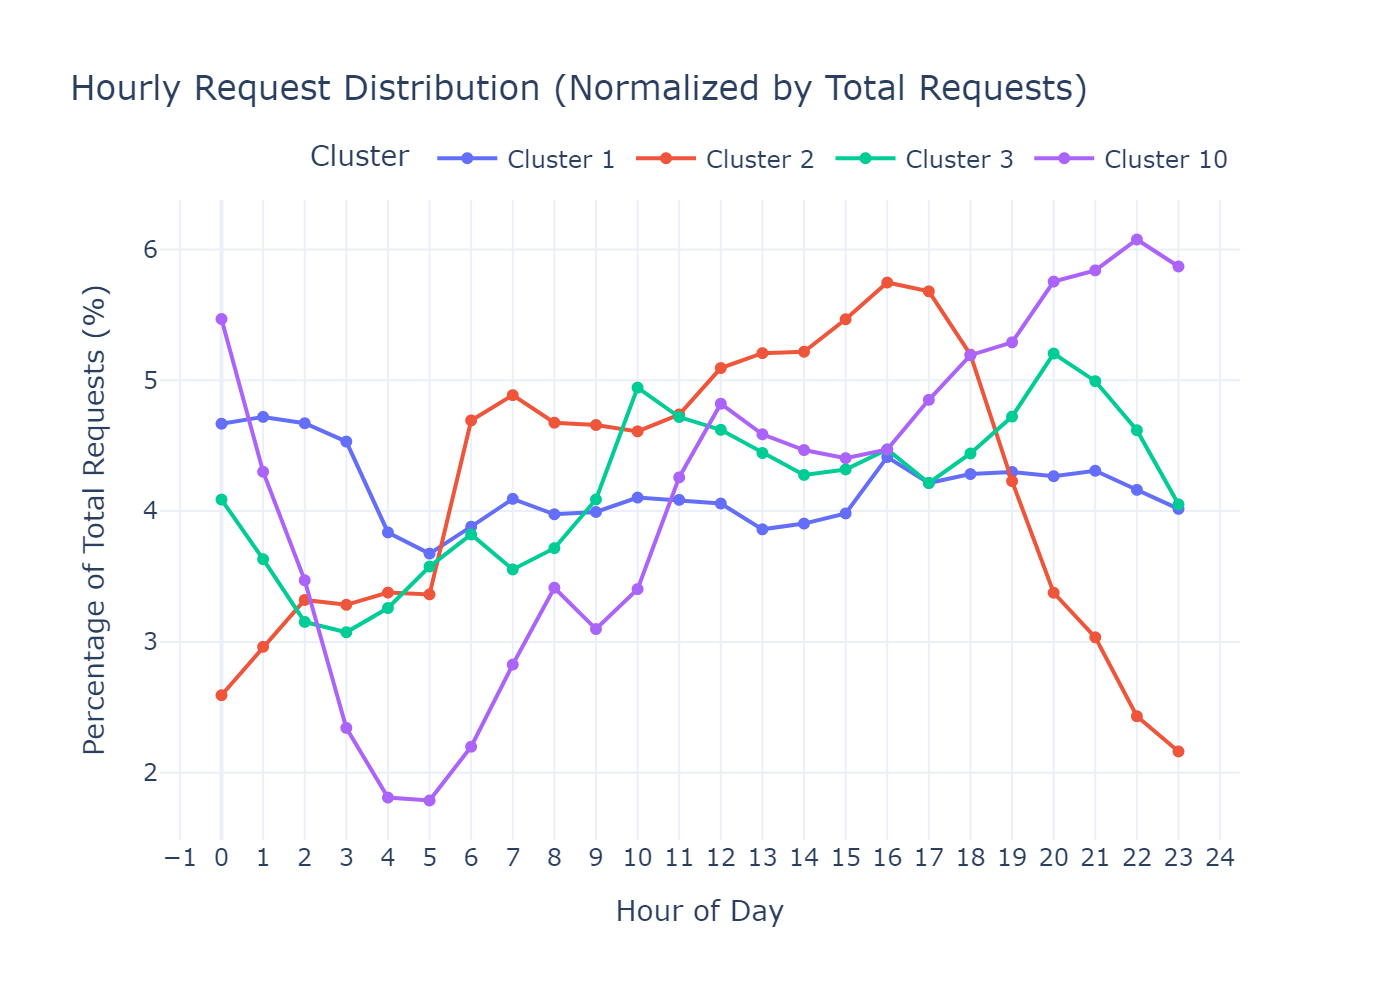
\includegraphics[width=1\linewidth]{visualizations/hourly_request_distribution.png}
    \caption{Hourly Request Distribution (Normalized by Total Requests)}
    \label{fig:hourly_request}
\end{figure}


\begin{itemize}
    \item Cluster 1 shows a relatively uniform distribution throughout the day, with slight increases during early morning hours (0-2) and evening hours (16-21).
    \item Cluster 2 exhibits a clear diurnal pattern, with peak activity during working hours (6-18) and significantly lower activity during night hours.
    \item Cluster 3 shows a bimodal distribution, with peaks around 10-11 AM and 20-21 PM.
    \item Cluster 10 displays a gradual increase in activity throughout the day, peaking in the evening hours (20-23).
\end{itemize}

These patterns suggest different use cases for each cluster. Cluster 1 might be serving a global user base with users distributed across time zones, resulting in a more uniform distribution. Cluster 2 appears to be serving a more localized user base with clear working hour patterns. Clusters 3 and 10 might be serving specific applications with usage patterns tied to certain times of day.

\subsection{Daily Request Distribution}
Figure \ref{fig:daily_request} shows the daily request distribution for all four clusters, normalized by total requests.

\begin{figure}[htbp]
    \centering
    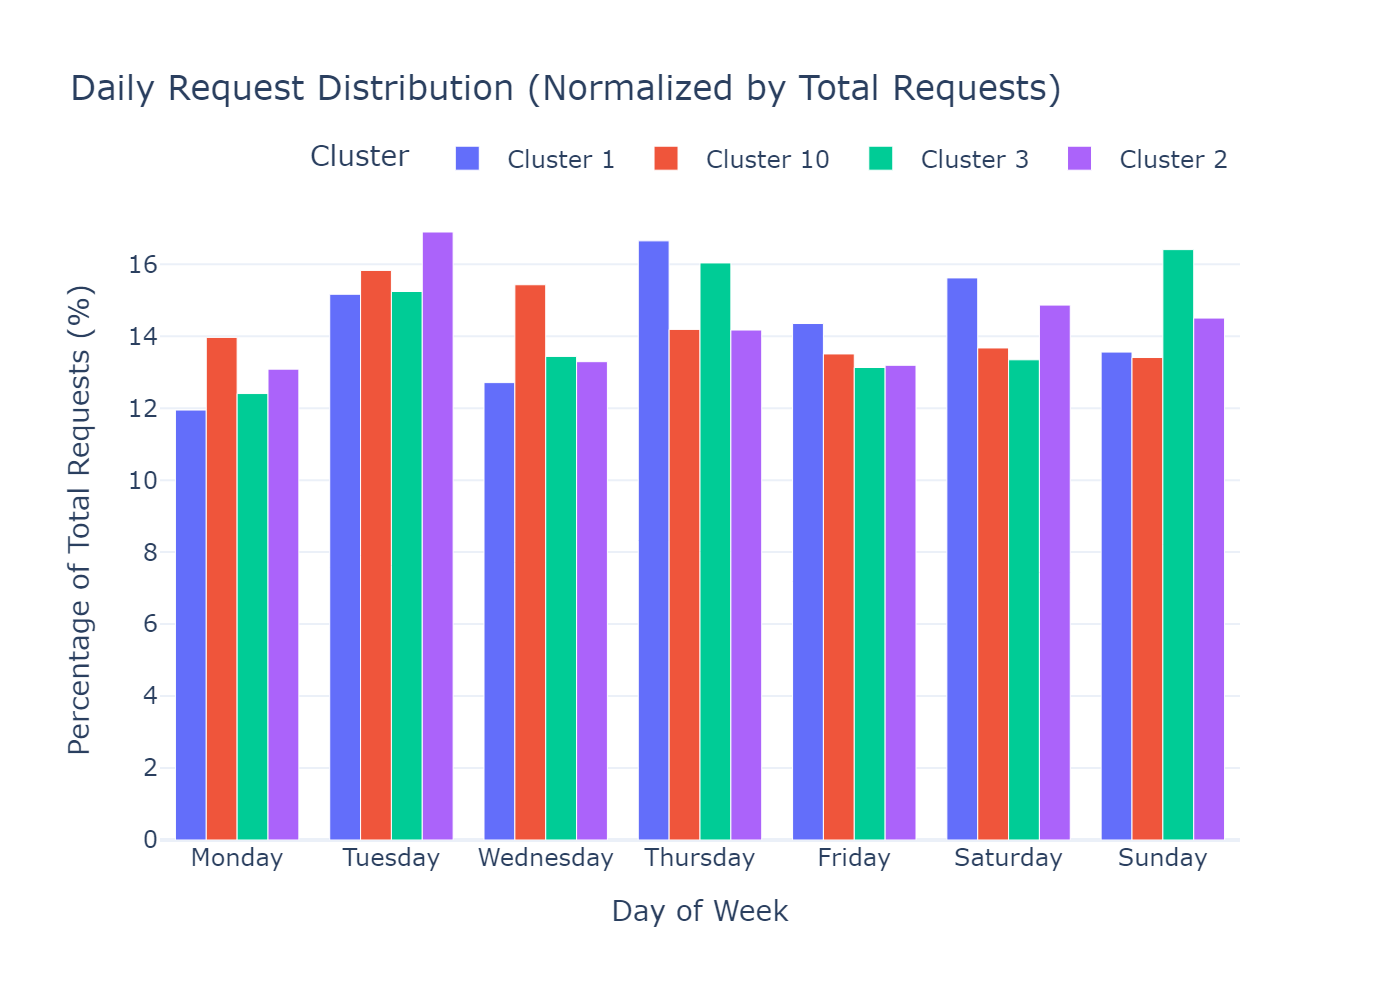
\includegraphics[width=1\linewidth]{visualizations/daily_request_distribution.png}
    \caption{Daily Request Distribution (Normalized by Total Requests)}
    \label{fig:daily_request}
\end{figure}

We observe the following patterns:
\begin{itemize}
    \item Cluster 1 shows higher activity on Tuesday, Thursday, and Saturday, with lower activity on Monday and Sunday.
    \item Cluster 2 has peak activity on Tuesday, with relatively consistent activity on other days.
    \item Cluster 3 shows highest activity on Thursday and Sunday, with lower activity on Monday.
    \item Cluster 10 has a more uniform distribution across days, with slightly higher activity on Tuesday.
\end{itemize}

These weekly patterns could reflect the nature of the services or applications being cached. For instance, social media features might see higher usage on weekends, while business applications might see higher usage on weekdays.

\subsection{Peak Period Analysis}
Figure \ref{fig:peak_period} shows the percentage of peak periods and the ratio of peak to non-peak traffic for each cluster.

\begin{figure}[htbp]
    \centering
    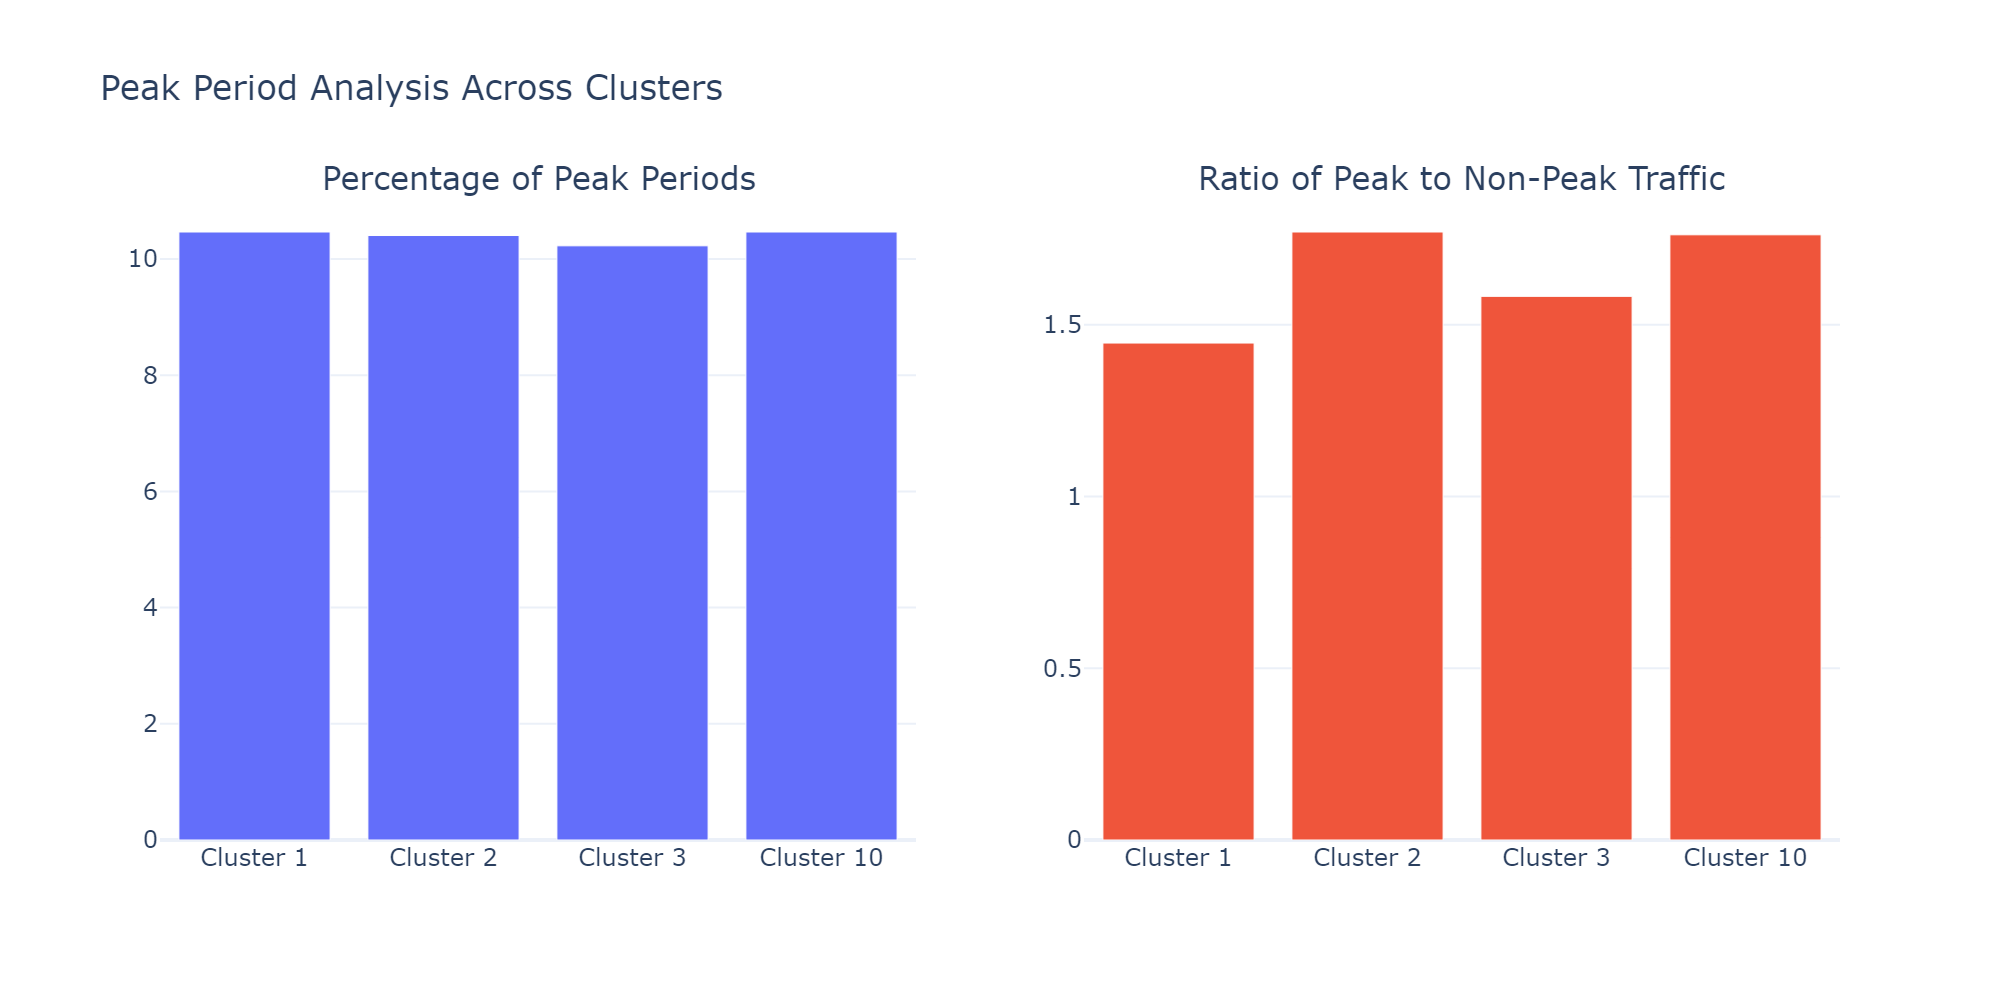
\includegraphics[width=1\linewidth]{visualizations/peak_period_analysis.png}
    \caption{Peak Period Analysis Across Clusters}
    \label{fig:peak_period}
\end{figure}

All clusters have a similar percentage of peak periods (around 10%), but the ratio of peak to non-peak traffic varies. Clusters 2 and 10 have the highest ratios (around 1.77), indicating more concentrated traffic during peak periods. Cluster 1 has the lowest ratio (1.45), suggesting a more even distribution of traffic.

Figure \ref{fig:peak_hour} shows the distribution of peak periods by hour of day.

\begin{figure}[htbp]
    \centering
    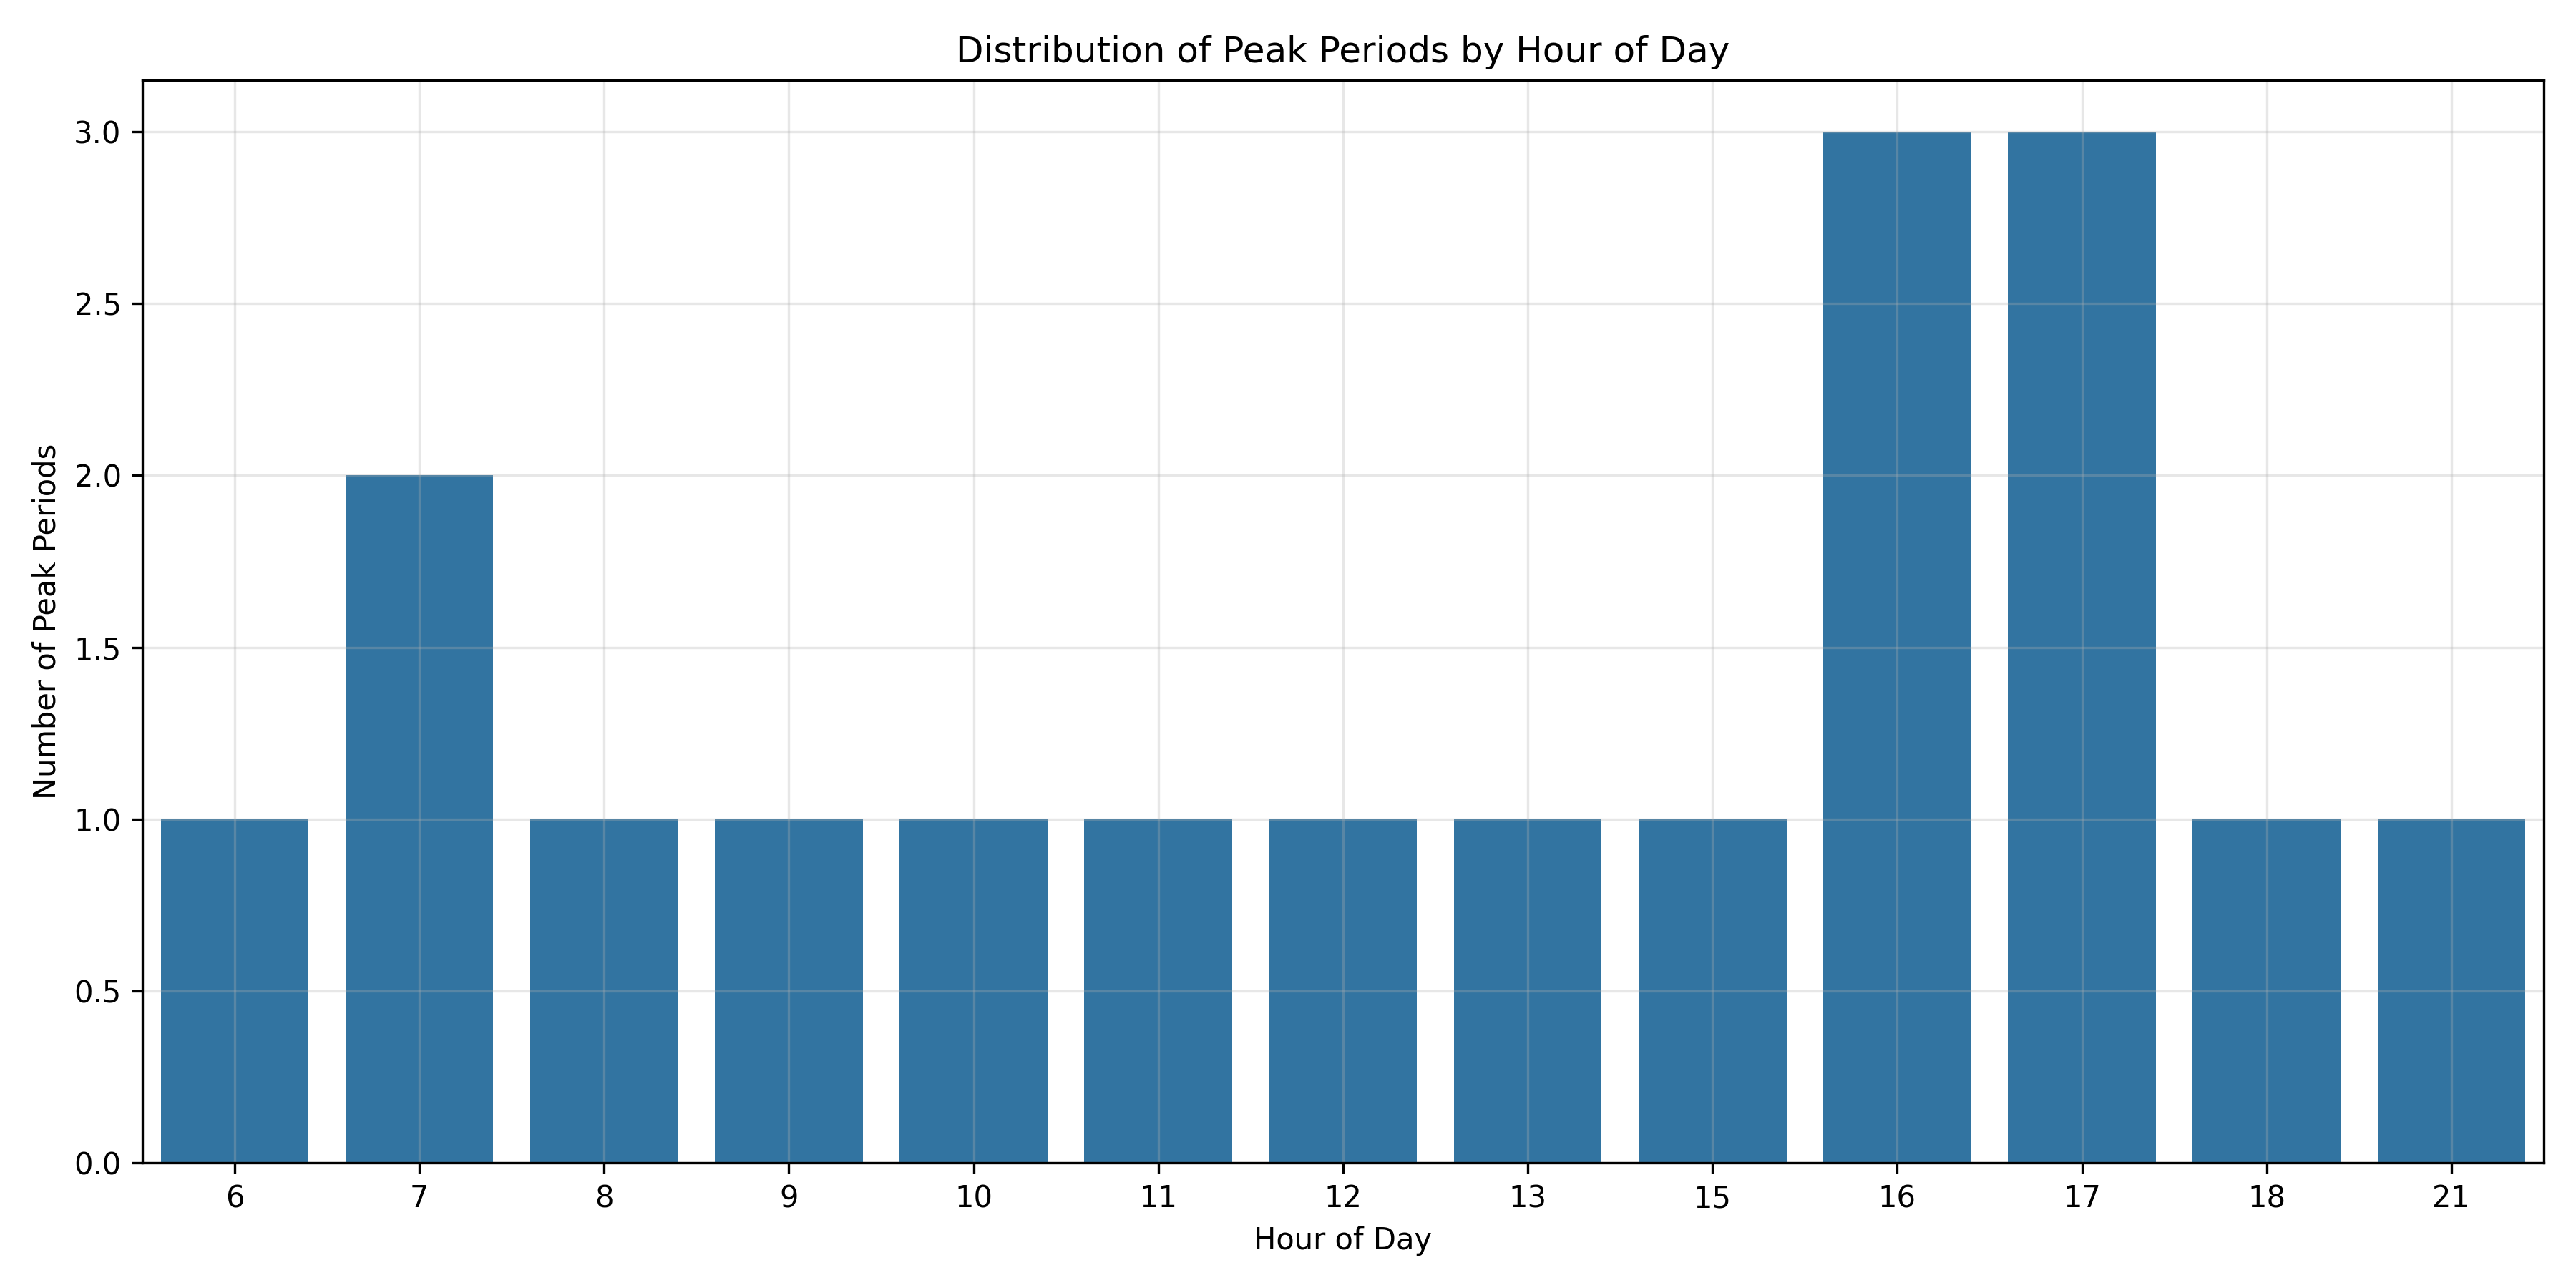
\includegraphics[width=\linewidth]{visualizations/peak_periods_by_hour.png}
    \caption{Distribution of Peak Periods by Hour of Day}
    \label{fig:peak_hour}
\end{figure}

Peak periods occur at different times for different clusters:
\begin{itemize}
    \item Cluster 1 has peak periods distributed throughout the day, with no clear pattern.
    \item Cluster 2 has most peak periods during working hours (7-18), with a concentration around 16-17.
    \item Cluster 3 has peaks around 10 AM and 20 PM, consistent with its bimodal hourly distribution.
    \item Cluster 10 has most peak periods in the evening (20-23).
\end{itemize}

\subsection{Request Volume and Variability}
Figure \ref{fig:request_volume} compares the total request volume, daily average, and hourly average across clusters.

\begin{figure}[htbp]
    \centering
    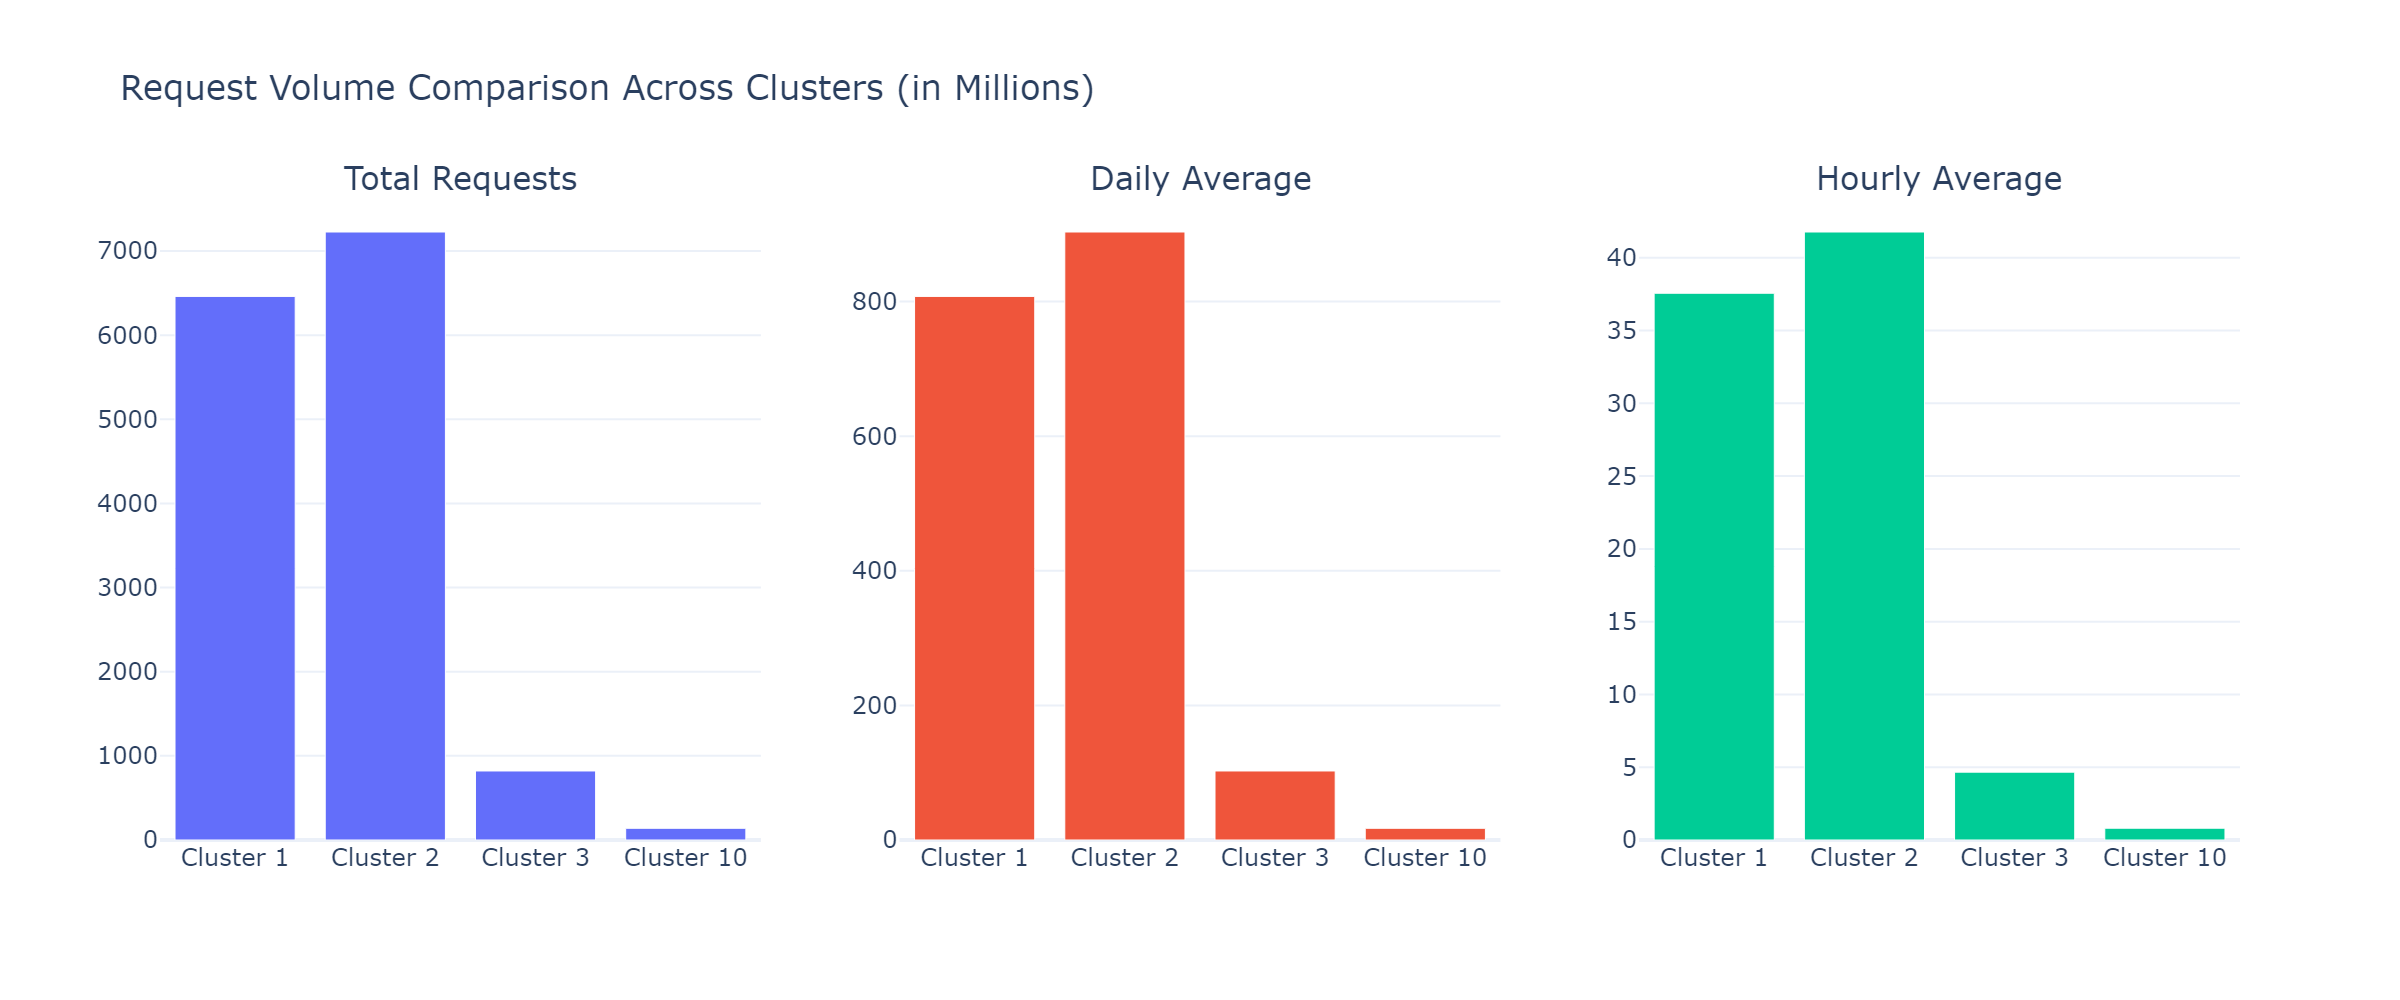
\includegraphics[width=\linewidth]{visualizations/request_volume_comparison.png}
    \caption{Request Volume Comparison Across Clusters (in Millions)}
    \label{fig:request_volume}
\end{figure}

Clusters 1 and 2 have the highest request volumes, with over 6 billion and 7 billion requests respectively. Cluster 3 has a moderate volume of around 820 million requests, while Cluster 10 has the lowest volume at around 139 million requests.

Figure \ref{fig:request_variability} shows the coefficient of variation and max/min ratio for hourly request volume.

\begin{figure}[htbp]
    \centering
    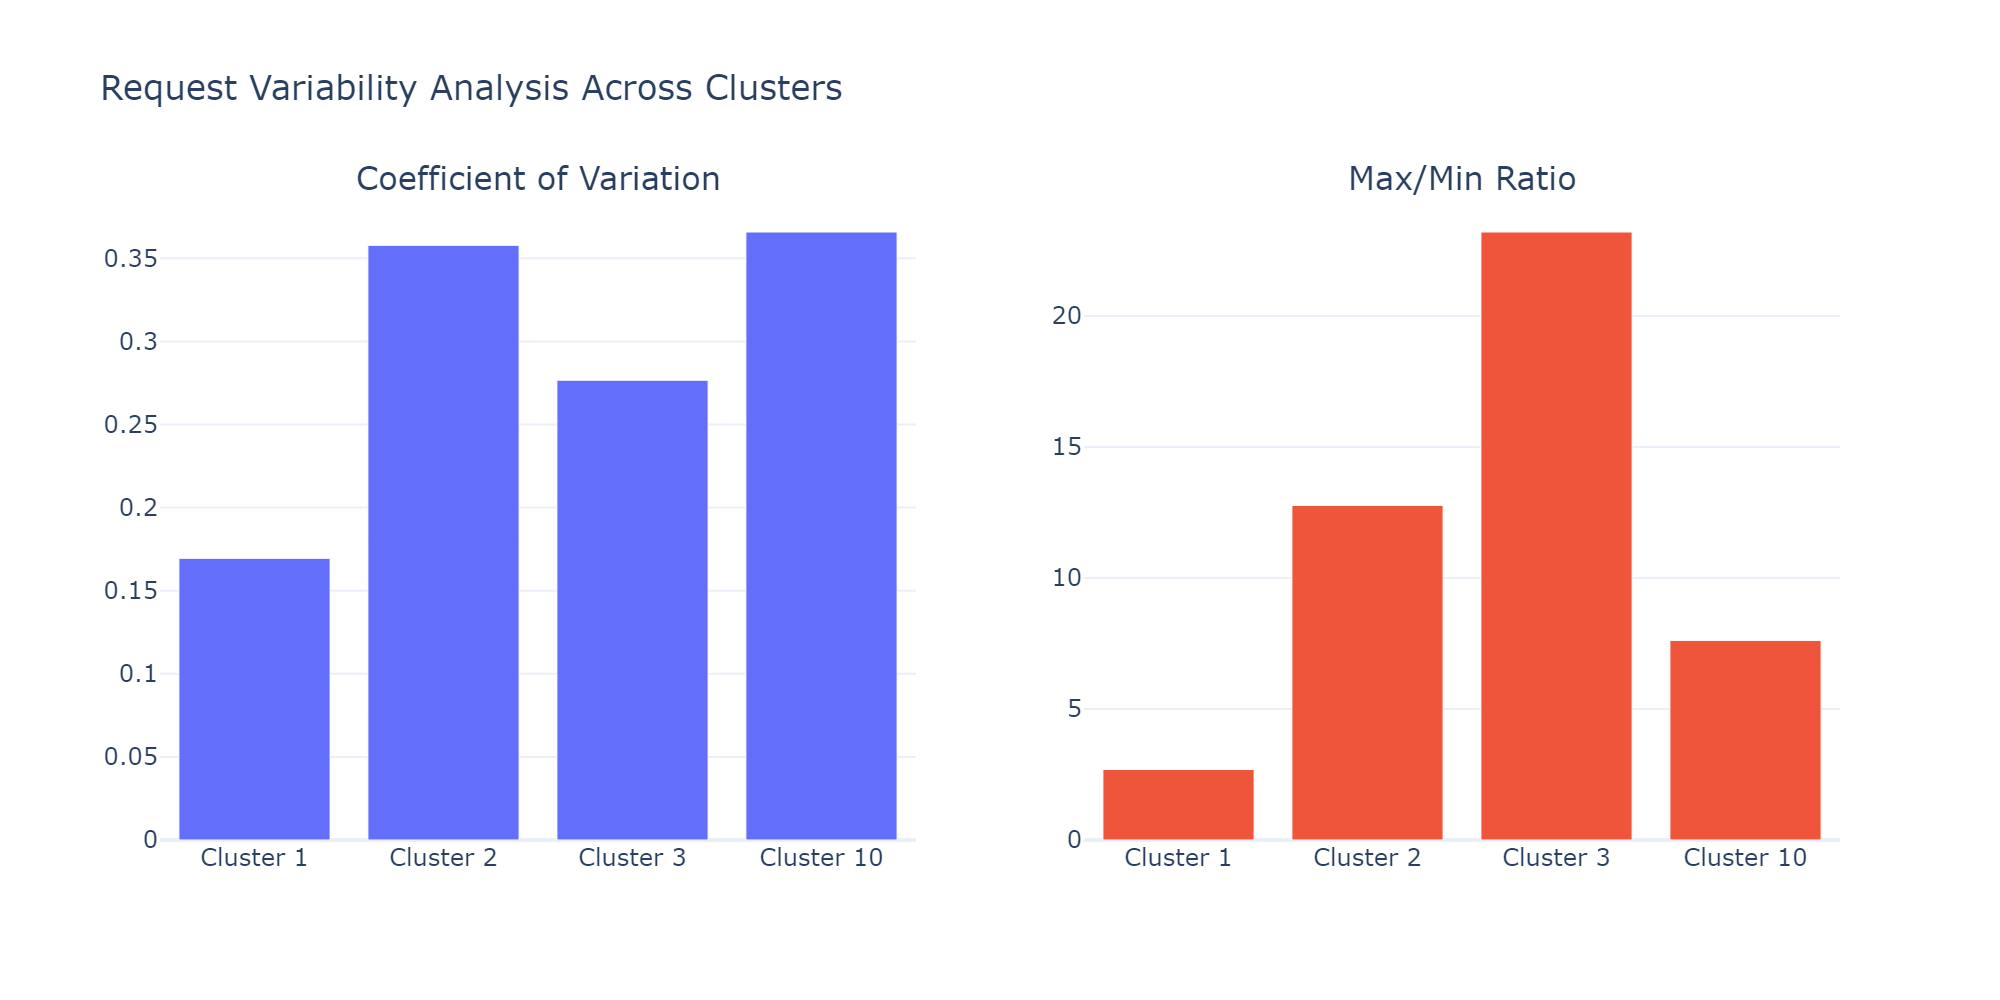
\includegraphics[width=\linewidth]{visualizations/request_variability_analysis.png}
    \caption{Request Variability Analysis Across Clusters}
    \label{fig:request_variability}
\end{figure}

Cluster 2 shows the highest variability, with a coefficient of variation of 0.36 and a max/min ratio of 12.77. This indicates significant fluctuations in request volume throughout the day. Cluster 1 has the lowest variability, with a coefficient of variation of 0.17 and a max/min ratio of 2.69, suggesting a more stable workload.

\section{Workload Composition Results}
This section presents our findings on workload composition across the four clusters.

\subsection{Operation Type Distribution}
Figure \ref{fig:operation_type} shows the distribution of operation types across clusters.

\begin{figure}[htbp]
    \centering
    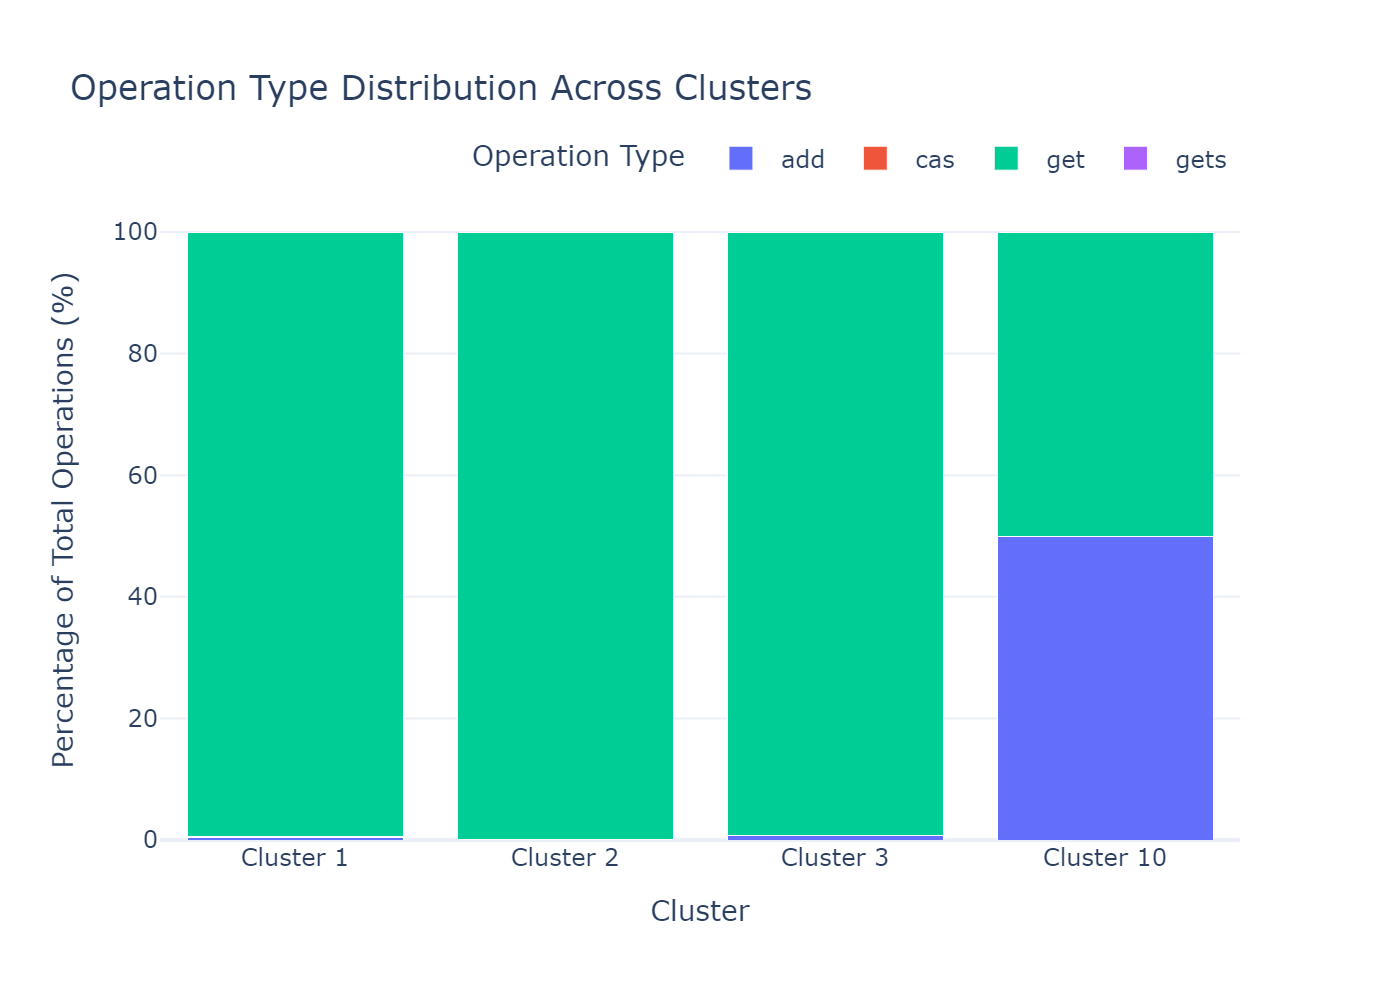
\includegraphics[width=\linewidth]{visualizations/operation_type_distribution.png}
    \caption{Operation Type Distribution Across Clusters}
    \label{fig:operation_type}
\end{figure}

We observe significant differences in operation type distribution:
\begin{itemize}
    \item Clusters 1, 2, and 3 are predominantly read-heavy, with get operations accounting for over 99\% of all operations.
    \item Cluster 10 has a balanced read-write workload, with approximately 50\% get operations and 50\% add operations.
\end{itemize}

This variation in workload composition has important implications for cache optimization. Read-heavy workloads might benefit from different replacement policies than balanced or write-heavy workloads.

\subsection{Key and Value Size Distribution}
Figure \ref{fig:key_size} shows the mean key size by operation type across clusters.

\begin{figure}[htbp]
    \centering
    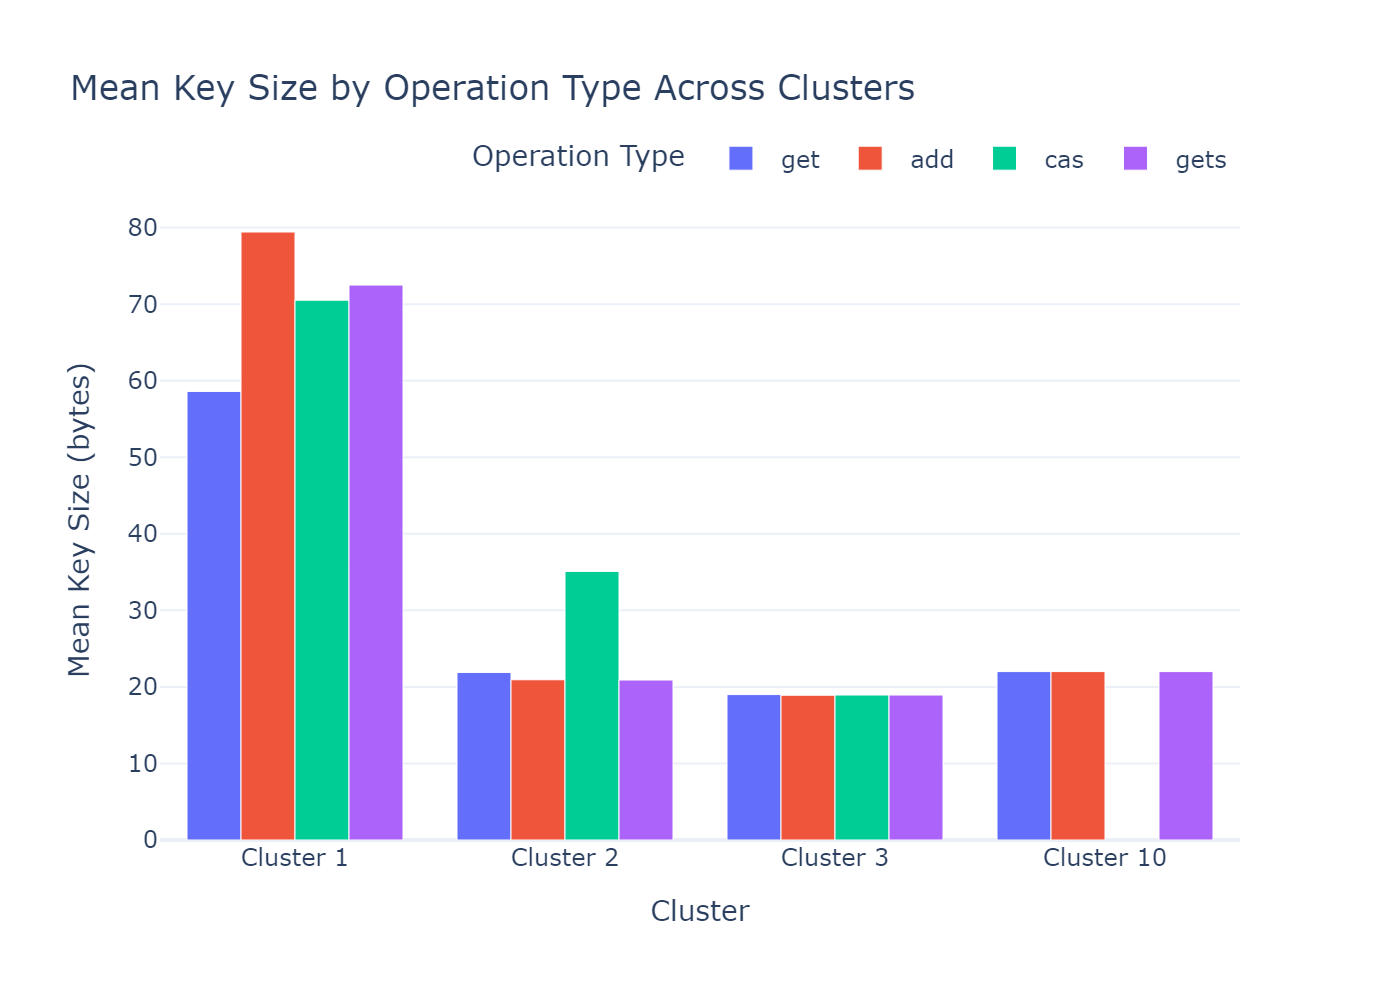
\includegraphics[width=\linewidth]{visualizations/key_size_distribution.png}
    \caption{Mean Key Size by Operation Type Across Clusters}
    \label{fig:key_size}
\end{figure}

Key sizes vary significantly across clusters:
\begin{itemize}
    \item Cluster 1 has the largest key sizes, with a mean of around 58-79 bytes depending on the operation type.
    \item Cluster 2 has smaller key sizes, with a mean of around 21 bytes.
    \item Cluster 3 has the smallest key sizes, with a mean of around 19 bytes.
    \item Cluster 10 has a uniform key size of 22 bytes for all operation types.
\end{itemize}

Figure \ref{fig:value_size} shows the value size statistics for add operations.

\begin{figure}[htbp]
\centering
    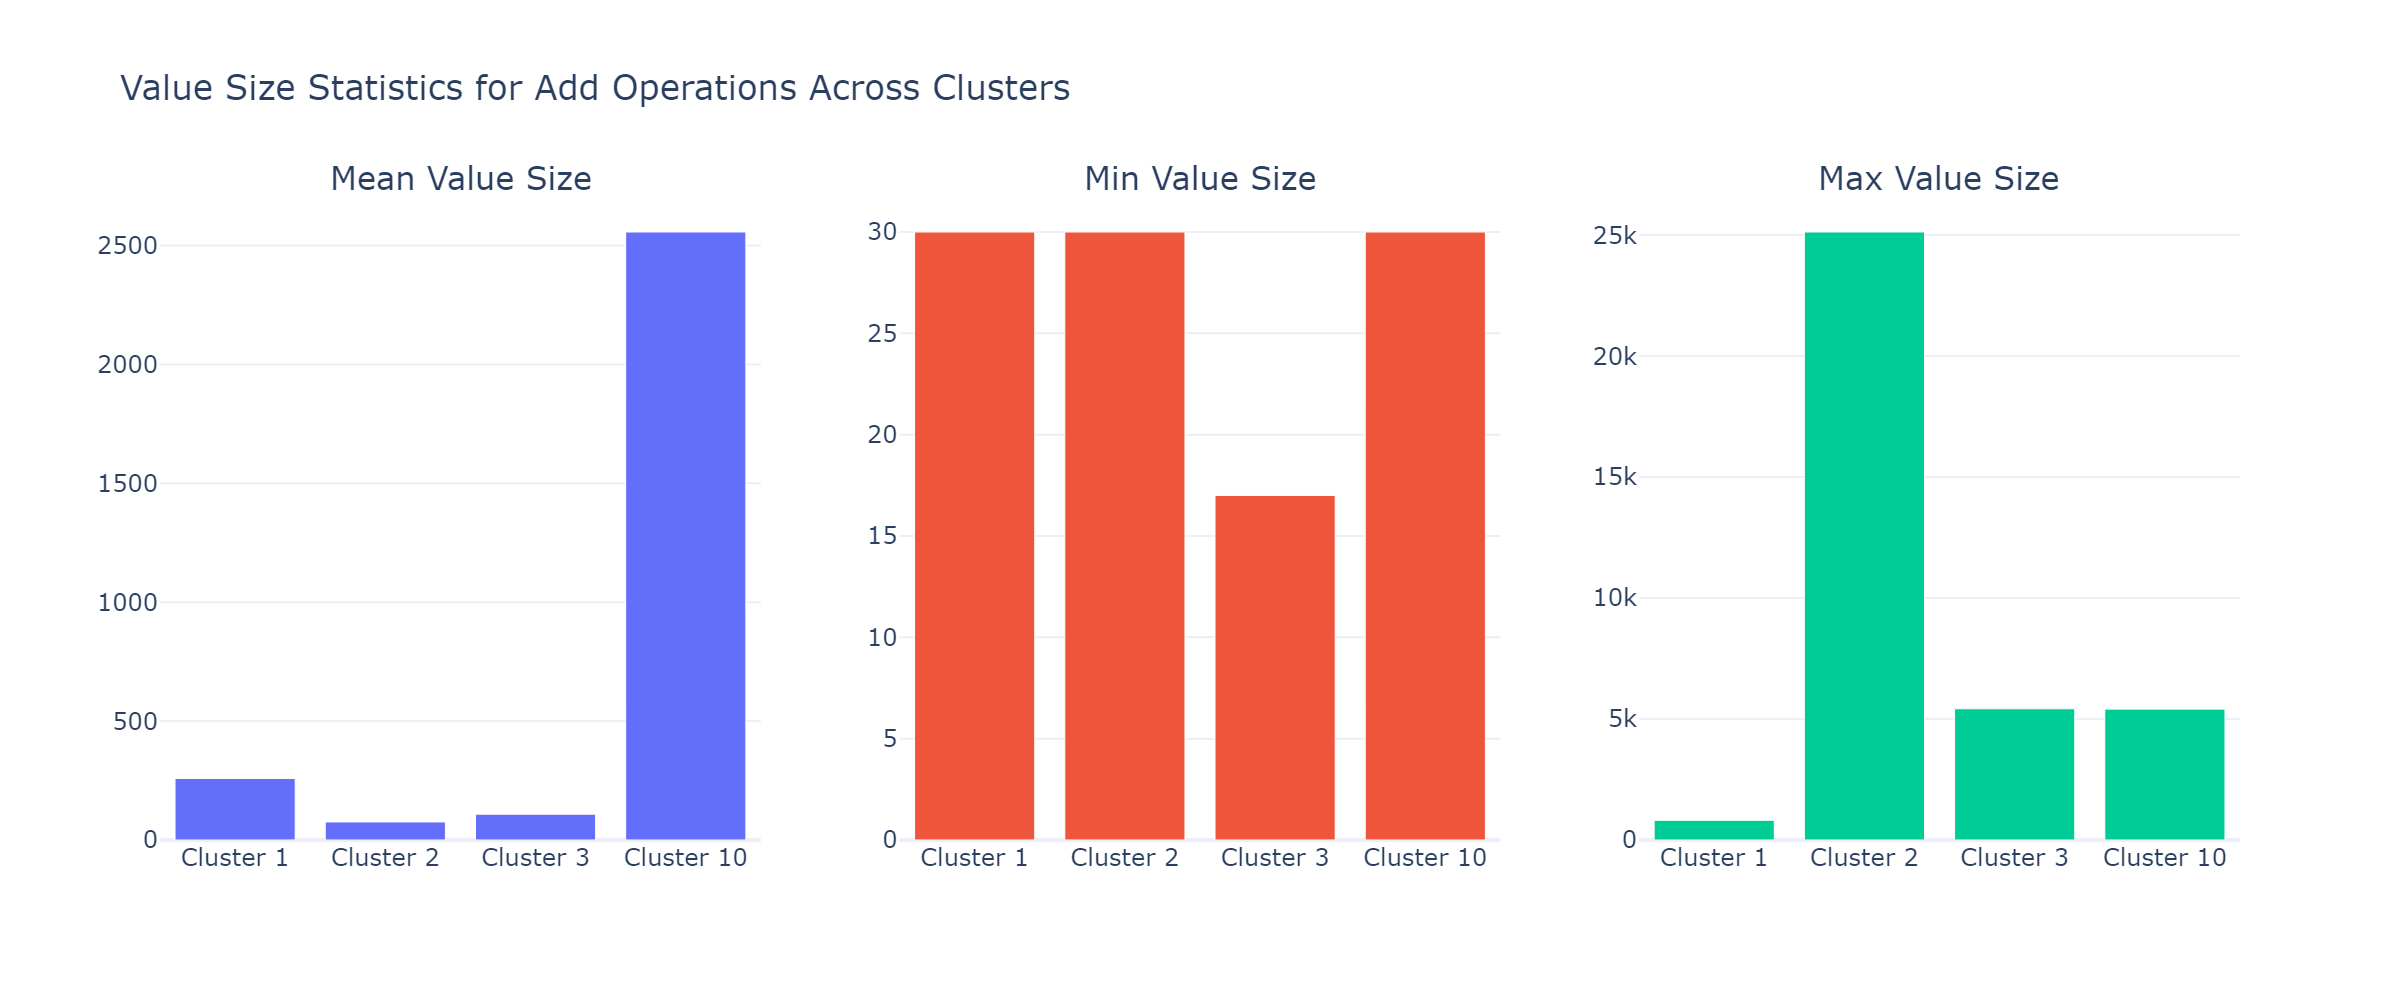
\includegraphics[width=\linewidth]{visualizations/value_size_distribution.png}
    \caption{Value Size Statistics for Add Operations Across Clusters}
    \label{fig:value_size}
\end{figure}

Value sizes also vary significantly:
\begin{itemize}
    \item Cluster 10 has the largest values, with a mean of over 2500 bytes.
    \item Cluster 1 has a mean value size of around 258 bytes.
    \item Clusters 2 and 3 have smaller values, with means of around 76 and 109 bytes respectively.
\end{itemize}

These differences in key and value sizes affect memory usage and can impact cache performance, particularly in terms of memory fragmentation and eviction efficiency.

\subsection{TTL Distribution}
Figure \ref{fig:ttl} shows the mean TTL for add operations across clusters.

\begin{figure}[htbp]
    \centering
    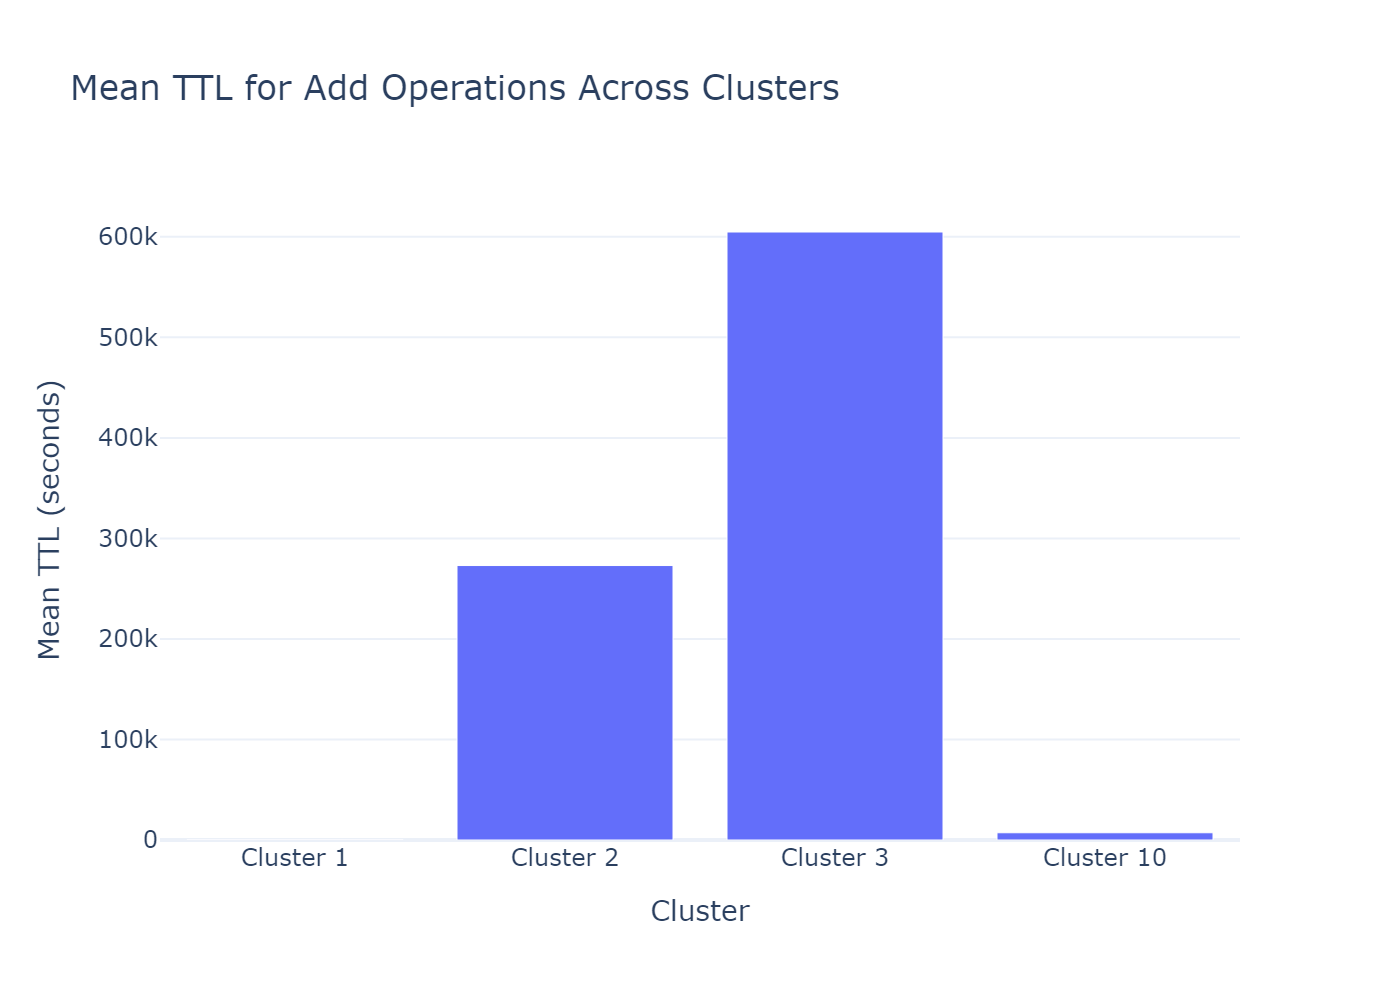
\includegraphics[width=\linewidth]{visualizations/ttl_distribution.png}
    \caption{Mean TTL for Add Operations Across Clusters}
    \label{fig:ttl}
\end{figure}

TTL values vary dramatically across clusters:
\begin{itemize}
    \item Cluster 3 has the longest TTL, with a mean of around 604,800 seconds (7 days).
    \item Cluster 2 has a mean TTL of around 273,022 seconds (3.16 days).
    \item Cluster 10 has a mean TTL of around 7,200 seconds (2 hours).
    \item Cluster 1 has the shortest TTL, with a mean of around 240 seconds (4 minutes).
\end{itemize}

These TTL differences suggest different caching strategies and requirements. Cluster 1's short TTL indicates a need for frequent updates, possibly due to rapidly changing data. Cluster 3's long TTL suggests more stable data that can be cached for extended periods.

\subsection{Daily Operation Trends}
Figure \ref{fig:daily_operation} shows the daily operation trends by cluster.

\begin{figure}[htbp]
    \centering
    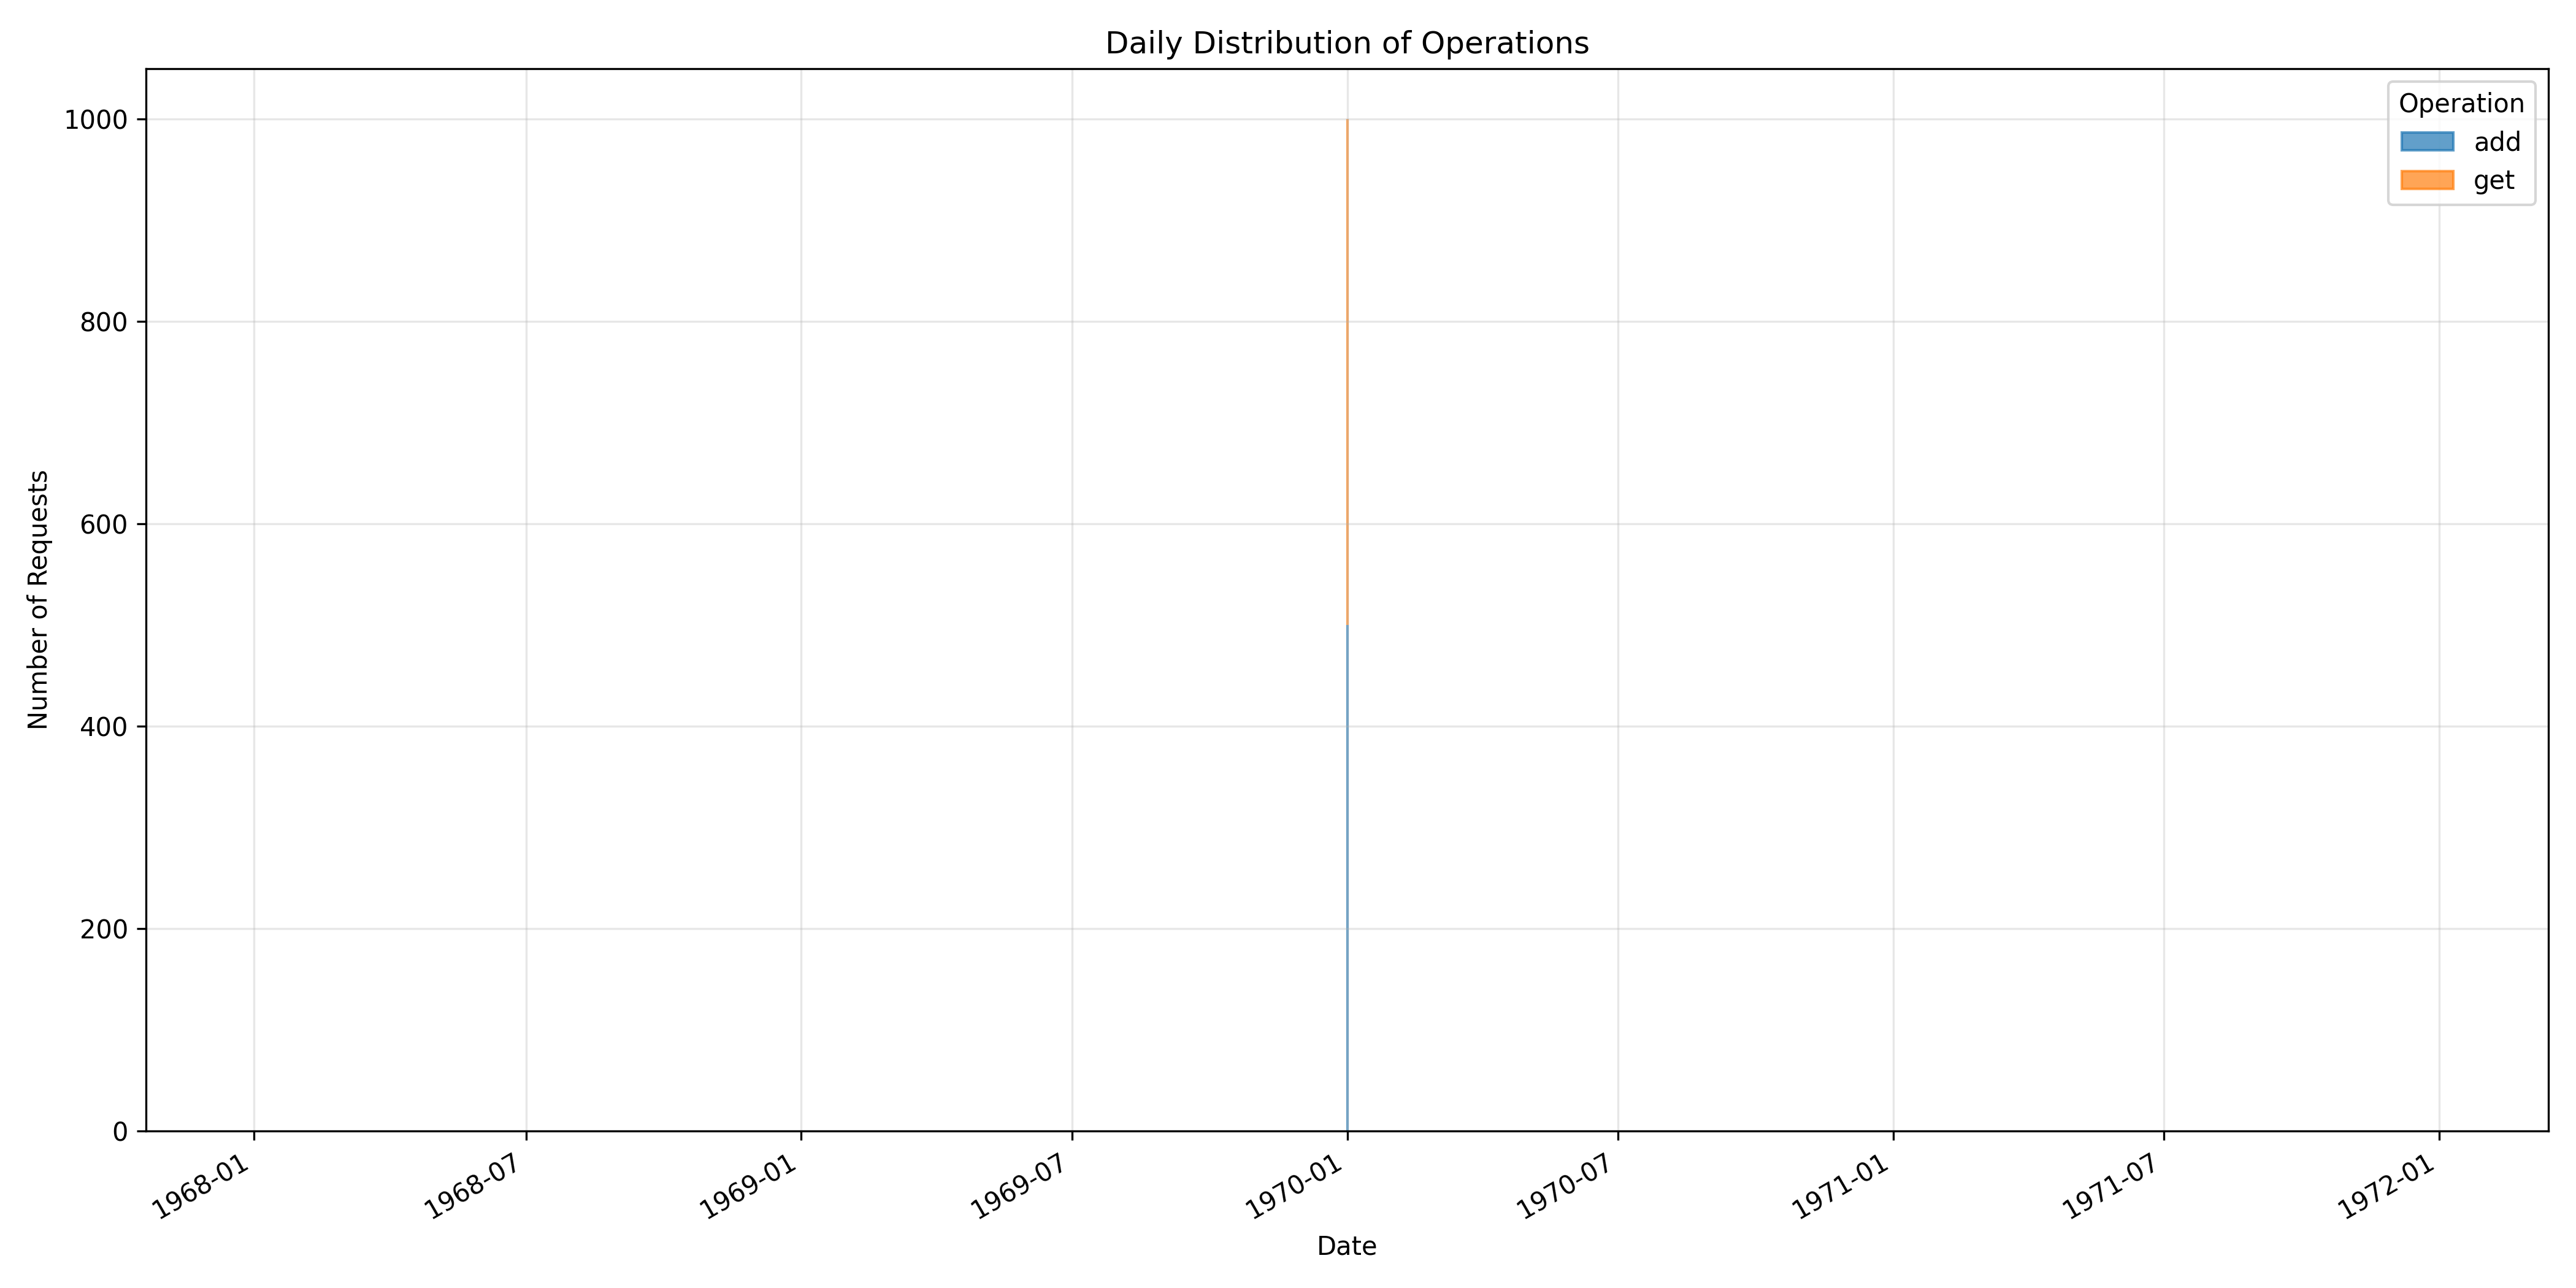
\includegraphics[width=\linewidth]{visualizations/daily_operation_trends.png}
    \caption{Daily Operation Trends by Cluster}
    \label{fig:daily_operation}
\end{figure}

The trends show relatively stable operation distributions over the week for all clusters, with some day-to-day variations. This stability suggests that while the overall request volume may vary by day, the proportion of different operations remains relatively consistent.

\subsection{Get/Add Ratio}
Figure \ref{fig:get_add_ratio} shows the ratio of get operations to add operations across clusters.

\begin{figure}[htbp]
    \centering
    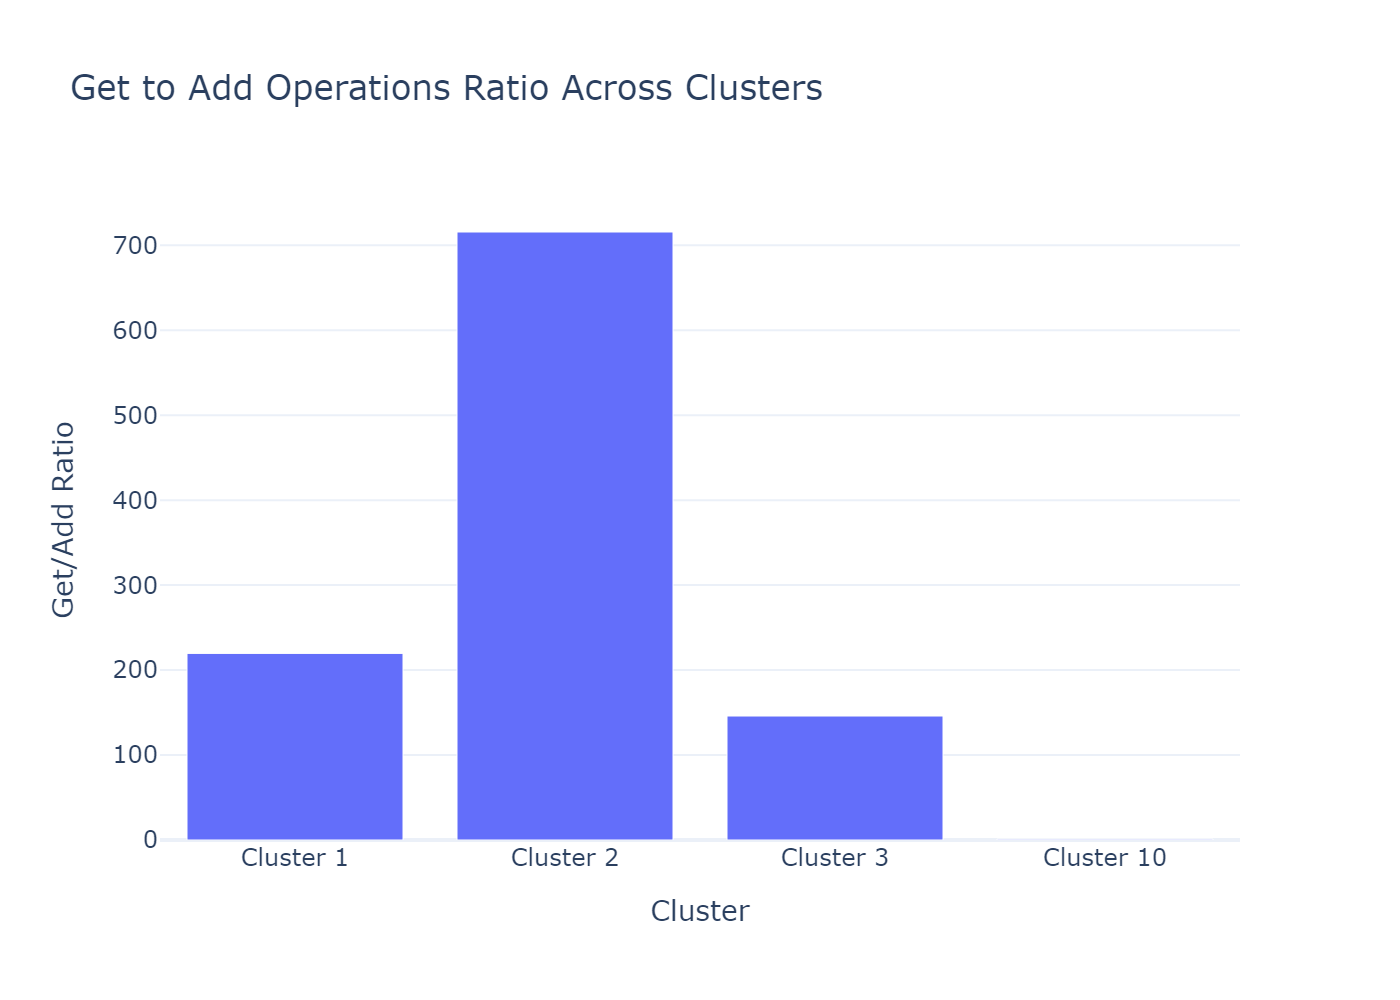
\includegraphics[width=\linewidth]{visualizations/get_add_ratio.png}
    \caption{Get to Add Operations Ratio Across Clusters}
    \label{fig:get_add_ratio}
\end{figure}

The get/add ratio varies dramatically:
\begin{itemize}
    \item Cluster 2 has the highest ratio at 715.65, indicating an extremely read-heavy workload.
    \item Cluster 1 has a ratio of 219.64, also indicating a read-heavy workload.
    \item Cluster 3 has a ratio of 145.93, still read-heavy but less extreme.
    \item Cluster 10 has a ratio of 1.00, indicating a perfectly balanced read-write workload.
\end{itemize}

These ratios provide insight into the nature of the cached data and how it's used. High ratios suggest data that is written once and read many times, while lower ratios indicate more frequent updates.

\section{Discussion}
Our analysis of cache access patterns and workload composition across four Twitter cache clusters reveals several insights that can inform cache optimization strategies.

\subsection{Implications for Cache Sizing}
The temporal patterns observed, particularly the hourly distributions and peak period analysis, have important implications for cache sizing. Clusters with high variability in request volume, such as Cluster 2, might benefit from dynamic cache sizing approaches that allocate more memory during peak periods and less during off-peak times. Conversely, clusters with more uniform distributions, such as Cluster 1, might be better served by static cache sizing.

The workload composition also affects cache sizing decisions. Clusters with larger key and value sizes, such as Cluster 1 for keys and Cluster 10 for values, require more memory per cached item. Additionally, the get/add ratio influences the rate at which new items are added to the cache, which in turn affects the cache size needed to maintain a target hit rate.

\subsection{Implications for Replacement Policies}
Our findings on workload composition, particularly the operation type distribution and get/add ratio, have implications for cache replacement policies. Traditional policies like LRU (Least Recently Used) are designed for read-heavy workloads and may not perform optimally for balanced workloads like that of Cluster 10.

For read-heavy workloads (Clusters 1, 2, and 3), LRU or variants like LRU-K might be appropriate. However, as noted in related work \cite{yang2021large}, FIFO can perform similarly to LRU under reasonable cache sizes, offering a simpler and potentially more efficient alternative.

For balanced workloads (Cluster 10), policies that consider both recency and frequency, such as ARC (Adaptive Replacement Cache) or LIRS (Low Inter-reference Recency Set), might be more effective. These policies can better handle the mix of read and write operations characteristic of such workloads.

\subsection{Implications for TTL Management}
The wide variation in TTL values across clusters highlights the importance of TTL management in cache optimization. Clusters with short TTLs, such as Cluster 1, require efficient mechanisms for removing expired items to maintain cache effectiveness. As noted in related work \cite{yang2021large}, efficiently removing expired objects should be prioritized over cache eviction.

For clusters with longer TTLs, such as Cluster 3, the focus might shift more towards optimizing for cache hits, as items remain valid for extended periods. However, even with long TTLs, it's important to consider the effective working set size, which is influenced by both TTL and access patterns.

\subsection{Implications for Multi-Cluster Optimization}
The significant differences observed across clusters suggest that a one-size-fits-all approach to cache optimization is unlikely to be effective. Instead, cache parameters and policies should be tailored to the specific characteristics of each cluster.

For organizations managing multiple cache clusters, our methodology provides a framework for analyzing and comparing cluster characteristics. This can inform decisions about which clusters might benefit from similar optimization strategies and which require distinct approaches.

\section{Bias Consideration}

In this section, we critically examine potential biases in the Twitter cache trace dataset and discuss how these biases might affect the generalizability of our findings to other cache systems and environments.

\subsection{Dataset Representation Bias}

The Twitter cache trace dataset, while extensive, represents a specific operational environment with particular characteristics that may not be universal across all cache deployments:

\begin{itemize}
    \item \textbf{Social Media Context}: The traces originate from Twitter's infrastructure, which serves a social media platform with specific access patterns driven by user behavior on that platform. These patterns may differ significantly from those in other domains such as e-commerce, content delivery networks, or enterprise applications.
    
    \item \textbf{Cluster Selection}: Our analysis focused on clusters 1, 2, 3, and 10, which represent only a subset of Twitter's cache infrastructure. The selection of these specific clusters may not capture the full diversity of cache workloads across the entire system.
    
    \item \textbf{Temporal Limitations}: The dataset captures a specific time period, which may not account for seasonal variations, evolving user behaviors, or significant platform events that could alter cache access patterns.
\end{itemize}

\subsection{Technical Bias}

Several technical factors in the dataset collection and processing may introduce biases:

\begin{itemize}
    \item \textbf{Timestamp Anonymization}: A critical bias in the dataset is that timestamps were anonymized to start at 0 (Unix epoch). This anonymization has several important implications:
    \begin{itemize}
        \item Loss of absolute temporal context, preventing correlation with external events or seasonal trends
        \item Uncertainty in day/week identification, as our mapping of timestamps to specific days or hours relies on assumptions
        \item Limitations in long-term trend analysis, as gradual shifts over real calendar time are obscured
        \item Challenges in cross-dataset comparison with traces that maintain real timestamps
    \end{itemize}
    While the relative patterns (daily and weekly cycles) may still be valid, the specific mapping to real-world time periods carries significant uncertainty.
    
    \item \textbf{Sampling Methodology}: The dataset was collected using a sampling approach rather than capturing all cache operations. The sampling rate and methodology could potentially over-represent or under-represent certain types of operations or time periods.
    
    \item \textbf{Anonymization Effects}: For privacy and security reasons, the dataset has been anonymized, with actual keys replaced with hashed values. This anonymization preserves key size and operation type but may obscure semantic patterns that could be relevant for certain analyses.
    
    \item \textbf{Cache Implementation Specifics}: The traces come from Twitter's Twemcache implementation, which has specific design choices and optimizations. These implementation details may influence the observed patterns in ways that would not generalize to other cache systems with different architectures.
\end{itemize}

\subsection{Impact on Generalizability}

These biases affect the generalizability of our findings in several important ways:

\begin{itemize}
    \item \textbf{Workload Composition}: While our analysis of operation types (get, add, set, delete) provides valuable insights, the specific distribution may be unique to Twitter's use case. Other systems might show dramatically different operation type distributions based on their application requirements.
    
    \item \textbf{Temporal Patterns}: The daily and weekly patterns we observed may be strongly influenced by Twitter's global user base and social media usage patterns. Systems serving different geographic regions or application domains may exhibit different temporal characteristics. Additionally, the timestamp anonymization means we cannot be certain about the exact alignment of these patterns with real-world time periods.
    
    \item \textbf{Size Distributions}: The key and value size distributions we analyzed may reflect Twitter's specific data models and content types. Other systems with different data structures would likely show different size distributions.
\end{itemize}

\subsection{Mitigation Strategies}

To address these biases and improve the generalizability of our findings, we recommend:

\begin{itemize}
    \item \textbf{Cross-Dataset Validation}: Comparing our findings with analyses of cache traces from different domains and systems would help identify which patterns are Twitter-specific and which are more universal.
    
    \item \textbf{Synthetic Workload Testing}: Developing synthetic workloads based on our findings but with parametric variations could help test the robustness of cache optimization strategies across a broader range of scenarios.
    
    \item \textbf{Longitudinal Studies}: Analyzing cache traces over longer time periods would help distinguish between stable patterns and temporary anomalies or trends.
    
    \item \textbf{Domain-Specific Contextualization}: When applying insights from this analysis to other systems, carefully considering the specific domain context and adjusting expectations accordingly.
    
    \item \textbf{Temporal Pattern Verification}: For future studies, if possible, obtaining non-anonymized timestamps or at least information about the mapping between anonymized and real timestamps would significantly improve the reliability of temporal analyses.
\end{itemize}

Despite these limitations, the Twitter cache trace dataset provides valuable real-world insights that can inform cache system design and optimization. By acknowledging these biases, we can more appropriately apply the findings to other contexts while recognizing where additional research or customization may be necessary.

\section{Conclusion}
In this paper, we analyzed cache access patterns and workload composition using publicly available Twitter cache traces from four different clusters. Our analysis revealed significant variations in both temporal patterns and workload composition across clusters, highlighting the importance of cluster-specific optimization strategies.

Key findings from our temporal analysis include:
\begin{itemize}
    \item Distinct hourly patterns across clusters, ranging from uniform distributions to clear diurnal patterns.
    \item Weekly patterns with varying levels of activity on different days.
    \item Significant differences in request variability, with some clusters showing much higher fluctuations than others.
\end{itemize}

Key findings from our workload composition analysis include:
\begin{itemize}
    \item Varying operation type distributions, from extremely read-heavy to balanced read-write workloads.
    \item Significant differences in key and value sizes across clusters.
    \item Wide variation in TTL values, from minutes to days.
    \item Get/add ratios ranging from 1.00 to over 700.
\end{itemize}

These findings have important implications for cache optimization strategies, including cache sizing, replacement policies, and TTL management. They suggest that cache parameters and policies should be tailored to the specific characteristics of each cluster, rather than applying a one-size-fits-all approach.

\subsection{Relevance}
This work demonstrates several key concepts central to storage systems design and optimization:
\begin{itemize}
    \item \textbf{Hierarchical Storage Management}: Our analysis highlights the critical role of in-memory caches as the fastest tier in modern storage hierarchies, showing how workload characteristics influence the effectiveness of this tier in reducing pressure on slower storage layers.
    
    \item \textbf{Workload-Aware System Design}: The significant variations in access patterns across clusters emphasize that storage systems must be designed with specific workload characteristics in mind, rather than assuming generic access patterns.
    
    \item \textbf{Temporal Locality Exploitation}: The temporal patterns identified in our analysis demonstrate how modern storage systems can leverage predictable access patterns to prefetch data and optimize resource allocation dynamically.
    
    \item \textbf{Size-Aware Caching}: Our findings on key and value size distributions illustrate the importance of considering object sizes in storage system design, particularly for systems that must efficiently manage memory resources.
    
    \item \textbf{Data Lifecycle Management}: The TTL analysis provides insights into how storage systems must handle data expiration and garbage collection, balancing freshness requirements with resource utilization.
\end{itemize}

These observations connect directly to fundamental storage systems concepts such as locality of reference, working set theory, and tiered storage design, making this analysis valuable for understanding how theoretical principles manifest in real-world production environments.

\subsection{Limitations and Future Work}
Our study has several limitations that could be addressed in future work:
\begin{itemize}
    \item We analyzed only four clusters out of the 54 available in the Twitter cache-trace repository. A more comprehensive analysis covering more clusters could reveal additional patterns and insights.
    
    \item The timestamp anonymization in the dataset (reset to start at Unix epoch 0) introduces uncertainty in our temporal interpretations. Without actual dates and times, we cannot correlate cache access patterns with external events or seasonal trends, and our mapping of timestamps to specific days or hours relies on assumptions that may not match reality.
    
    \item The dataset's social media context may limit generalizability to other domains such as e-commerce or enterprise applications, as access patterns are likely influenced by Twitter's specific user behavior patterns.
    
    \item Future work could employ more advanced statistical techniques and machine learning approaches to identify patterns and correlations.
\end{itemize}

Despite these limitations, our analysis provides valuable insights into real-world cache behavior that can inform cache system design and optimization. Future research should focus on cross-dataset validation, obtaining non-anonymized temporal data when possible, and developing more robust methods for analyzing cache traces that account for the biases inherent in production datasets.


\begin{thebibliography}{00}
\bibitem{yang2021large} J. Yang, Y. Yue, and K. V. Rashmi, "A Large-scale Analysis of Hundreds of In-memory Key-value Cache Clusters at Twitter," ACM Trans. Storage, vol. 17, no. 3, Article 17, Aug. 2021.

\bibitem{qiu2023frozenhot} Z. Qiu et al., "FrozenHot Cache: Rethinking Cache Management for Modern Hardware," in Proc. 18th European Conference on Computer Systems (EuroSys '23), May 2023, pp. 1-17.

\bibitem{twitter_cache_trace} "Twitter Cache Trace," GitHub repository, https://github.com/twitter/cache-trace.

\bibitem{cidon2016cliffhanger} A. Cidon et al., "Cliffhanger: Scaling Performance Cliffs in Web Memory Caches," in Proc. 13th USENIX Symposium on Networked Systems Design and Implementation (NSDI '16), Mar. 2016, pp. 379-392.

\bibitem{blankstein2017hyperbolic} A. Blankstein, S. Sen, and M. J. Freedman, "Hyperbolic Caching: Flexible Caching for Web Applications," in Proc. USENIX Annual Technical Conference (USENIX ATC '17), Jul. 2017, pp. 499-511.

\bibitem{narayanan2008write} D. Narayanan, A. Donnelly, and A. Rowstron, "Write Off-Loading: Practical Power Management for Enterprise Storage," ACM Trans. Storage, vol. 4, no. 3, Article 10, Nov. 2008.

\bibitem{cao2020characterizing} Z. Cao et al., "Characterizing, Modeling, and Benchmarking RocksDB Key-Value Workloads at Facebook," in Proc. 18th USENIX Conference on File and Storage Technologies (FAST '20), Feb. 2020, pp. 209-223.
\end{thebibliography}

\end{document}
